\documentclass[1p]{elsarticle_modified}
%\bibliographystyle{elsarticle-num}

%\usepackage[colorlinks]{hyperref}
%\usepackage{abbrmath_seonhwa} %\Abb, \Ascr, \Acal ,\Abf, \Afrak
\usepackage{amsfonts}
\usepackage{amssymb}
\usepackage{amsmath}
\usepackage{amsthm}
\usepackage{scalefnt}
\usepackage{amsbsy}
\usepackage{kotex}
\usepackage{caption}
\usepackage{subfig}
\usepackage{color}
\usepackage{graphicx}
\usepackage{xcolor} %% white, black, red, green, blue, cyan, magenta, yellow
\usepackage{float}
\usepackage{setspace}
\usepackage{hyperref}

\usepackage{tikz}
\usetikzlibrary{arrows}

\usepackage{multirow}
\usepackage{array} % fixed length table
\usepackage{hhline}

%%%%%%%%%%%%%%%%%%%%%
\makeatletter
\renewcommand*\env@matrix[1][\arraystretch]{%
	\edef\arraystretch{#1}%
	\hskip -\arraycolsep
	\let\@ifnextchar\new@ifnextchar
	\array{*\c@MaxMatrixCols c}}
\makeatother %https://tex.stackexchange.com/questions/14071/how-can-i-increase-the-line-spacing-in-a-matrix
%%%%%%%%%%%%%%%

\usepackage[normalem]{ulem}

\newcommand{\msout}[1]{\ifmmode\text{\sout{\ensuremath{#1}}}\else\sout{#1}\fi}
%SOURCE: \msout is \stkout macro in https://tex.stackexchange.com/questions/20609/strikeout-in-math-mode

\newcommand{\cancel}[1]{
	\ifmmode
	{\color{red}\msout{#1}}
	\else
	{\color{red}\sout{#1}}
	\fi
}

\newcommand{\add}[1]{
	{\color{blue}\uwave{#1}}
}

\newcommand{\replace}[2]{
	\ifmmode
	{\color{red}\msout{#1}}{\color{blue}\uwave{#2}}
	\else
	{\color{red}\sout{#1}}{\color{blue}\uwave{#2}}
	\fi
}

\newcommand{\Sol}{\mathcal{S}} %segment
\newcommand{\D}{D} %diagram
\newcommand{\A}{\mathcal{A}} %arc


%%%%%%%%%%%%%%%%%%%%%%%%%%%%%5 test

\def\sl{\operatorname{\textup{SL}}(2,\Cbb)}
\def\psl{\operatorname{\textup{PSL}}(2,\Cbb)}
\def\quan{\mkern 1mu \triangleright \mkern 1mu}

\theoremstyle{definition}
\newtheorem{thm}{Theorem}[section]
\newtheorem{prop}[thm]{Proposition}
\newtheorem{lem}[thm]{Lemma}
\newtheorem{ques}[thm]{Question}
\newtheorem{cor}[thm]{Corollary}
\newtheorem{defn}[thm]{Definition}
\newtheorem{exam}[thm]{Example}
\newtheorem{rmk}[thm]{Remark}
\newtheorem{alg}[thm]{Algorithm}

\newcommand{\I}{\sqrt{-1}}
\begin{document}

%\begin{frontmatter}
%
%\title{Boundary parabolic representations of knots up to 8 crossings}
%
%%% Group authors per affiliation:
%\author{Yunhi Cho} 
%\address{Department of Mathematics, University of Seoul, Seoul, Korea}
%\ead{yhcho@uos.ac.kr}
%
%
%\author{Seonhwa Kim} %\fnref{s_kim}}
%\address{Center for Geometry and Physics, Institute for Basic Science, Pohang, 37673, Korea}
%\ead{ryeona17@ibs.re.kr}
%
%\author{Hyuk Kim}
%\address{Department of Mathematical Sciences, Seoul National University, Seoul 08826, Korea}
%\ead{hyukkim@snu.ac.kr}
%
%\author{Seokbeom Yoon}
%\address{Department of Mathematical Sciences, Seoul National University, Seoul, 08826,  Korea}
%\ead{sbyoon15@snu.ac.kr}
%
%\begin{abstract}
%We find all boundary parabolic representation of knots up to 8 crossings.
%
%\end{abstract}
%\begin{keyword}
%    \MSC[2010] 57M25 
%\end{keyword}
%
%\end{frontmatter}

%\linenumbers
%\tableofcontents
%
\newcommand\colored[1]{\textcolor{white}{\rule[-0.35ex]{0.8em}{1.4ex}}\kern-0.8em\color{red} #1}%
%\newcommand\colored[1]{\textcolor{white}{ #1}\kern-2.17ex	\textcolor{white}{ #1}\kern-1.81ex	\textcolor{white}{ #1}\kern-2.15ex\color{red}#1	}

{\Large $\underline{10_{69}~(K10a_{38})}$}

\setlength{\tabcolsep}{10pt}
\renewcommand{\arraystretch}{1.6}
\vspace{1cm}\begin{tabular}{m{100pt}>{\centering\arraybackslash}m{274pt}}
\multirow{5}{120pt}{
	\centering
	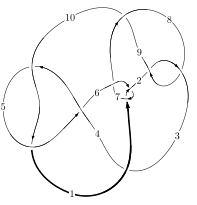
\includegraphics[width=112pt]{../../../GIT/diagram.site/Diagrams/png/153_10_69.png}\\
\ \ \ A knot diagram\footnotemark}&
\allowdisplaybreaks
\textbf{Linearized knot diagam} \\
\cline{2-2}
 &
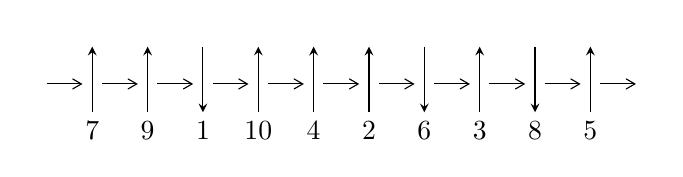
\begin{tikzpicture}[x=20pt, y=17pt]
	% nodes
	\node (C0) at (0, 0) {};
	\node (C1) at (1, 0) {};
	\node (C1U) at (1, +1) {};
	\node (C1D) at (1, -1) {7};

	\node (C2) at (2, 0) {};
	\node (C2U) at (2, +1) {};
	\node (C2D) at (2, -1) {9};

	\node (C3) at (3, 0) {};
	\node (C3U) at (3, +1) {};
	\node (C3D) at (3, -1) {1};

	\node (C4) at (4, 0) {};
	\node (C4U) at (4, +1) {};
	\node (C4D) at (4, -1) {10};

	\node (C5) at (5, 0) {};
	\node (C5U) at (5, +1) {};
	\node (C5D) at (5, -1) {4};

	\node (C6) at (6, 0) {};
	\node (C6U) at (6, +1) {};
	\node (C6D) at (6, -1) {2};

	\node (C7) at (7, 0) {};
	\node (C7U) at (7, +1) {};
	\node (C7D) at (7, -1) {6};

	\node (C8) at (8, 0) {};
	\node (C8U) at (8, +1) {};
	\node (C8D) at (8, -1) {3};

	\node (C9) at (9, 0) {};
	\node (C9U) at (9, +1) {};
	\node (C9D) at (9, -1) {8};

	\node (C10) at (10, 0) {};
	\node (C10U) at (10, +1) {};
	\node (C10D) at (10, -1) {5};
	\node (C11) at (11, 0) {};

	% arrows
	\draw[->,>={angle 60}]
	(C0) edge (C1) (C1) edge (C2) (C2) edge (C3) (C3) edge (C4) (C4) edge (C5) (C5) edge (C6) (C6) edge (C7) (C7) edge (C8) (C8) edge (C9) (C9) edge (C10) (C10) edge (C11) ;	\draw[->,>=stealth]
	(C1D) edge (C1U) (C2D) edge (C2U) (C3U) edge (C3D) (C4D) edge (C4U) (C5D) edge (C5U) (C6D) edge (C6U) (C7U) edge (C7D) (C8D) edge (C8U) (C9U) edge (C9D) (C10D) edge (C10U) ;
	\end{tikzpicture} \\
\hhline{~~} \\& 
\textbf{Solving Sequence} \\ \cline{2-2} 
 &
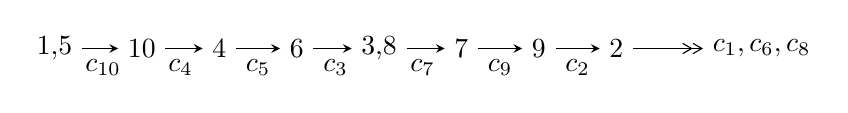
\begin{tikzpicture}[x=28pt, y=7pt]
	% node
	\node (A0) at (-1/8, 0) {1,5};
	\node (A1) at (1, 0) {10};
	\node (A2) at (2, 0) {4};
	\node (A3) at (3, 0) {6};
	\node (A4) at (65/16, 0) {3,8};
	\node (A5) at (41/8, 0) {7};
	\node (A6) at (49/8, 0) {9};
	\node (A7) at (57/8, 0) {2};
	\node (C1) at (1/2, -1) {$c_{10}$};
	\node (C2) at (3/2, -1) {$c_{4}$};
	\node (C3) at (5/2, -1) {$c_{5}$};
	\node (C4) at (7/2, -1) {$c_{3}$};
	\node (C5) at (37/8, -1) {$c_{7}$};
	\node (C6) at (45/8, -1) {$c_{9}$};
	\node (C7) at (53/8, -1) {$c_{2}$};
	\node (A8) at (9, 0) {$c_{1},c_{6},c_{8}$};

	% edge
	\draw[->,>=stealth]	
	(A0) edge (A1) (A1) edge (A2) (A2) edge (A3) (A3) edge (A4) (A4) edge (A5) (A5) edge (A6) (A6) edge (A7) ;
	\draw[->>,>={angle 60}]	
	(A7) edge (A8);
\end{tikzpicture} \\ 

\end{tabular} \\

\footnotetext{
The image of knot diagram is generated by the software ``\textbf{Draw programme}" developed by Andrew Bartholomew(\url{http://www.layer8.co.uk/maths/draw/index.htm\#Running-draw}), where we modified some parts for our purpose(\url{https://github.com/CATsTAILs/LinksPainter}).
}\phantom \\ \newline 
\centering \textbf{Ideals for irreducible components\footnotemark of $X_{\text{par}}$} 
 
\begin{align*}
I^u_{1}&=\langle 
- u^{18}-3 u^{17}+\cdots+b-3,\;-3 u^{18}-7 u^{17}+\cdots+2 a-7,\;u^{19}+3 u^{18}+\cdots+7 u+2\rangle \\
I^u_{2}&=\langle 
4 u^{13} a-17 u^{13}+\cdots+a+22,\;2 u^{13} a-2 u^{13}+\cdots-2 a+2,\\
\phantom{I^u_{2}}&\phantom{= \langle  }u^{14}- u^{13}-3 u^{12}+4 u^{11}+4 u^{10}-7 u^9- u^8+6 u^7-2 u^6-2 u^5+2 u^4- u+1\rangle \\
I^u_{3}&=\langle 
u^3+b,\;u^2+a+u-1,\;u^4- u^2+1\rangle \\
\\
\end{align*}
\raggedright * 3 irreducible components of $\dim_{\mathbb{C}}=0$, with total 51 representations.\\
\footnotetext{All coefficients of polynomials are rational numbers. But the coefficients are sometimes approximated in decimal forms when there is not enough margin.}
\newpage
\renewcommand{\arraystretch}{1}
\centering \section*{I. $I^u_{1}= \langle - u^{18}-3 u^{17}+\cdots+b-3,\;-3 u^{18}-7 u^{17}+\cdots+2 a-7,\;u^{19}+3 u^{18}+\cdots+7 u+2 \rangle$}
\flushleft \textbf{(i) Arc colorings}\\
\begin{tabular}{m{7pt} m{180pt} m{7pt} m{180pt} }
\flushright $a_{1}=$&$\begin{pmatrix}1\\0\end{pmatrix}$ \\
\flushright $a_{5}=$&$\begin{pmatrix}0\\u\end{pmatrix}$ \\
\flushright $a_{10}=$&$\begin{pmatrix}1\\u^2\end{pmatrix}$ \\
\flushright $a_{4}=$&$\begin{pmatrix}- u\\- u^3+u\end{pmatrix}$ \\
\flushright $a_{6}=$&$\begin{pmatrix}u^3\\u^5- u^3+u\end{pmatrix}$ \\
\flushright $a_{3}=$&$\begin{pmatrix}- u^3\\- u^3+u\end{pmatrix}$ \\
\flushright $a_{8}=$&$\begin{pmatrix}\frac{3}{2} u^{18}+\frac{7}{2} u^{17}+\cdots+\frac{17}{2} u+\frac{7}{2}\\u^{18}+3 u^{17}+\cdots+8 u+3\end{pmatrix}$ \\
\flushright $a_{7}=$&$\begin{pmatrix}\frac{1}{2} u^{18}+\frac{3}{2} u^{17}+\cdots+\frac{7}{2} u+\frac{3}{2}\\u^{17}+u^{16}+\cdots+2 u+1\end{pmatrix}$ \\
\flushright $a_{9}=$&$\begin{pmatrix}-\frac{1}{2} u^{18}-\frac{3}{2} u^{17}+\cdots-\frac{7}{2} u-\frac{1}{2}\\- u^{17}- u^{16}+\cdots-3 u-1\end{pmatrix}$ \\
\flushright $a_{2}=$&$\begin{pmatrix}\frac{3}{2} u^{18}+\frac{7}{2} u^{17}+\cdots+\frac{17}{2} u+\frac{7}{2}\\- u^{18}-2 u^{17}+\cdots-4 u-1\end{pmatrix}$\\&\end{tabular}
\flushleft \textbf{(ii) Obstruction class $= -1$}\\~\\
\flushleft \textbf{(iii) Cusp Shapes $= 12 u^{18}+26 u^{17}-24 u^{16}-116 u^{15}-42 u^{14}+200 u^{13}+222 u^{12}-116 u^{11}-334 u^{10}-108 u^9+228 u^8+240 u^7-4 u^6-172 u^5-118 u^4+12 u^3+78 u^2+64 u+30$}\\~\\
\newpage\renewcommand{\arraystretch}{1}
\flushleft \textbf{(iv) u-Polynomials at the component}\newline \\
\begin{tabular}{m{50pt}|m{274pt}}
Crossings & \hspace{64pt}u-Polynomials at each crossing \\
\hline $$\begin{aligned}c_{1},c_{2},c_{6}\\c_{8}\end{aligned}$$&$\begin{aligned}
&u^{19}+4 u^{17}+\cdots+2 u-1
\end{aligned}$\\
\hline $$\begin{aligned}c_{3}\end{aligned}$$&$\begin{aligned}
&u^{19}-9 u^{18}+\cdots+157 u-22
\end{aligned}$\\
\hline $$\begin{aligned}c_{4},c_{10}\end{aligned}$$&$\begin{aligned}
&u^{19}-3 u^{18}+\cdots+7 u-2
\end{aligned}$\\
\hline $$\begin{aligned}c_{5}\end{aligned}$$&$\begin{aligned}
&u^{19}-9 u^{18}+\cdots+5 u-4
\end{aligned}$\\
\hline $$\begin{aligned}c_{7},c_{9}\end{aligned}$$&$\begin{aligned}
&u^{19}+8 u^{18}+\cdots-2 u-1
\end{aligned}$\\
\hline
\end{tabular}\\~\\
\newpage\renewcommand{\arraystretch}{1}
\flushleft \textbf{(v) Riley Polynomials at the component}\newline \\
\begin{tabular}{m{50pt}|m{274pt}}
Crossings & \hspace{64pt}Riley Polynomials at each crossing \\
\hline $$\begin{aligned}c_{1},c_{2},c_{6}\\c_{8}\end{aligned}$$&$\begin{aligned}
&y^{19}+8 y^{18}+\cdots-2 y-1
\end{aligned}$\\
\hline $$\begin{aligned}c_{3}\end{aligned}$$&$\begin{aligned}
&y^{19}+3 y^{18}+\cdots+1461 y-484
\end{aligned}$\\
\hline $$\begin{aligned}c_{4},c_{10}\end{aligned}$$&$\begin{aligned}
&y^{19}-9 y^{18}+\cdots+5 y-4
\end{aligned}$\\
\hline $$\begin{aligned}c_{5}\end{aligned}$$&$\begin{aligned}
&y^{19}+3 y^{18}+\cdots+129 y-16
\end{aligned}$\\
\hline $$\begin{aligned}c_{7},c_{9}\end{aligned}$$&$\begin{aligned}
&y^{19}+12 y^{18}+\cdots+30 y-1
\end{aligned}$\\
\hline
\end{tabular}\\~\\
\newpage\flushleft \textbf{(vi) Complex Volumes and Cusp Shapes}
$$\begin{array}{c|c|c}  
\text{Solutions to }I^u_{1}& \I (\text{vol} + \sqrt{-1}CS) & \text{Cusp shape}\\
 \hline 
\begin{aligned}
u &= -0.656620 + 0.736849 I \\
a &= -0.530916 + 0.111769 I \\
b &= -0.692991 - 0.514666 I\end{aligned}
 & -3.87251 - 6.01197 I & -0.18591 + 7.59122 I \\ \hline\begin{aligned}
u &= -0.656620 - 0.736849 I \\
a &= -0.530916 - 0.111769 I \\
b &= -0.692991 + 0.514666 I\end{aligned}
 & -3.87251 + 6.01197 I & -0.18591 - 7.59122 I \\ \hline\begin{aligned}
u &= \phantom{-}0.833011 + 0.594872 I \\
a &= \phantom{-}0.493073 - 0.284708 I \\
b &= \phantom{-}0.042413 + 0.483034 I\end{aligned}
 & -1.75185 + 2.35707 I & \phantom{-}4.45005 - 4.73717 I \\ \hline\begin{aligned}
u &= \phantom{-}0.833011 - 0.594872 I \\
a &= \phantom{-}0.493073 + 0.284708 I \\
b &= \phantom{-}0.042413 - 0.483034 I\end{aligned}
 & -1.75185 - 2.35707 I & \phantom{-}4.45005 + 4.73717 I \\ \hline\begin{aligned}
u &= -0.342490 + 0.822016 I \\
a &= -0.423303 - 0.244228 I \\
b &= -0.84616 + 1.72998 I\end{aligned}
 & -2.12081 + 8.87474 I & \phantom{-}0.63360 - 6.11132 I \\ \hline\begin{aligned}
u &= -0.342490 - 0.822016 I \\
a &= -0.423303 + 0.244228 I \\
b &= -0.84616 - 1.72998 I\end{aligned}
 & -2.12081 - 8.87474 I & \phantom{-}0.63360 + 6.11132 I \\ \hline\begin{aligned}
u &= -0.954304 + 0.656562 I \\
a &= \phantom{-}1.022240 + 0.645581 I \\
b &= \phantom{-}0.517413 - 0.115037 I\end{aligned}
 & -2.99077 + 0.72249 I & \phantom{-}1.52455 - 2.82827 I \\ \hline\begin{aligned}
u &= -0.954304 - 0.656562 I \\
a &= \phantom{-}1.022240 - 0.645581 I \\
b &= \phantom{-}0.517413 + 0.115037 I\end{aligned}
 & -2.99077 - 0.72249 I & \phantom{-}1.52455 + 2.82827 I \\ \hline\begin{aligned}
u &= \phantom{-}1.178790 + 0.200823 I \\
a &= \phantom{-}1.12805 + 1.83215 I \\
b &= -0.06929 + 1.61595 I\end{aligned}
 & \phantom{-}2.86306 - 5.96190 I & \phantom{-}6.84845 + 4.63798 I \\ \hline\begin{aligned}
u &= \phantom{-}1.178790 - 0.200823 I \\
a &= \phantom{-}1.12805 - 1.83215 I \\
b &= -0.06929 - 1.61595 I\end{aligned}
 & \phantom{-}2.86306 + 5.96190 I & \phantom{-}6.84845 - 4.63798 I\\
 \hline 
 \end{array}$$\newpage$$\begin{array}{c|c|c}  
\text{Solutions to }I^u_{1}& \I (\text{vol} + \sqrt{-1}CS) & \text{Cusp shape}\\
 \hline 
\begin{aligned}
u &= \phantom{-}1.160320 + 0.382174 I \\
a &= -0.30429 - 1.44141 I \\
b &= \phantom{-}0.996422 - 0.904006 I\end{aligned}
 & \phantom{-}5.16612 + 4.98291 I & \phantom{-}9.41511 - 6.18167 I \\ \hline\begin{aligned}
u &= \phantom{-}1.160320 - 0.382174 I \\
a &= -0.30429 + 1.44141 I \\
b &= \phantom{-}0.996422 + 0.904006 I\end{aligned}
 & \phantom{-}5.16612 - 4.98291 I & \phantom{-}9.41511 + 6.18167 I \\ \hline\begin{aligned}
u &= -1.141050 + 0.480142 I \\
a &= \phantom{-}0.96822 - 1.32852 I \\
b &= -0.00563 - 1.67007 I\end{aligned}
 & \phantom{-}4.50851 - 3.09886 I & \phantom{-}9.38086 + 1.28227 I \\ \hline\begin{aligned}
u &= -1.141050 - 0.480142 I \\
a &= \phantom{-}0.96822 + 1.32852 I \\
b &= -0.00563 + 1.67007 I\end{aligned}
 & \phantom{-}4.50851 + 3.09886 I & \phantom{-}9.38086 - 1.28227 I \\ \hline\begin{aligned}
u &= -1.143800 + 0.588812 I \\
a &= -1.12767 + 2.25574 I \\
b &= \phantom{-}0.96492 + 2.22818 I\end{aligned}
 & \phantom{-}0.26882 - 14.12650 I & \phantom{-}3.54919 + 9.60559 I \\ \hline\begin{aligned}
u &= -1.143800 - 0.588812 I \\
a &= -1.12767 - 2.25574 I \\
b &= \phantom{-}0.96492 - 2.22818 I\end{aligned}
 & \phantom{-}0.26882 + 14.12650 I & \phantom{-}3.54919 - 9.60559 I \\ \hline\begin{aligned}
u &= -0.085864 + 0.693927 I \\
a &= \phantom{-}0.667057 + 0.203041 I \\
b &= -0.176244 - 0.940079 I\end{aligned}
 & \phantom{-}1.57783 - 1.22058 I & \phantom{-}5.73688 + 3.21713 I \\ \hline\begin{aligned}
u &= -0.085864 - 0.693927 I \\
a &= \phantom{-}0.667057 - 0.203041 I \\
b &= -0.176244 + 0.940079 I\end{aligned}
 & \phantom{-}1.57783 + 1.22058 I & \phantom{-}5.73688 - 3.21713 I \\ \hline\begin{aligned}
u &= -0.695977\phantom{ +0.000000I} \\
a &= \phantom{-}0.715081\phantom{ +0.000000I} \\
b &= \phantom{-}0.538288\phantom{ +0.000000I}\end{aligned}
 & \phantom{-}0.927841\phantom{ +0.000000I} & \phantom{-}11.2940\phantom{ +0.000000I}\\
 \hline 
 \end{array}$$\newpage\newpage\renewcommand{\arraystretch}{1}
\centering \section*{II. $I^u_{2}= \langle 4 u^{13} a-17 u^{13}+\cdots+a+22,\;2 u^{13} a-2 u^{13}+\cdots-2 a+2,\;u^{14}- u^{13}+\cdots- u+1 \rangle$}
\flushleft \textbf{(i) Arc colorings}\\
\begin{tabular}{m{7pt} m{180pt} m{7pt} m{180pt} }
\flushright $a_{1}=$&$\begin{pmatrix}1\\0\end{pmatrix}$ \\
\flushright $a_{5}=$&$\begin{pmatrix}0\\u\end{pmatrix}$ \\
\flushright $a_{10}=$&$\begin{pmatrix}1\\u^2\end{pmatrix}$ \\
\flushright $a_{4}=$&$\begin{pmatrix}- u\\- u^3+u\end{pmatrix}$ \\
\flushright $a_{6}=$&$\begin{pmatrix}u^3\\u^5- u^3+u\end{pmatrix}$ \\
\flushright $a_{3}=$&$\begin{pmatrix}- u^3\\- u^3+u\end{pmatrix}$ \\
\flushright $a_{8}=$&$\begin{pmatrix}a\\-0.190476 a u^{13}+0.809524 u^{13}+\cdots-0.0476190 a-1.04762\end{pmatrix}$ \\
\flushright $a_{7}=$&$\begin{pmatrix}-0.190476 a u^{13}-0.190476 u^{13}+\cdots+0.952381 a-0.0476190\\0.190476 a u^{13}+0.190476 u^{13}+\cdots+0.0476190 a-0.952381\end{pmatrix}$ \\
\flushright $a_{9}=$&$\begin{pmatrix}-0.190476 a u^{13}-0.190476 u^{13}+\cdots+0.952381 a-0.0476190\\-0.619048 a u^{13}+0.380952 u^{13}+\cdots+0.0952381 a-0.904762\end{pmatrix}$ \\
\flushright $a_{2}=$&$\begin{pmatrix}-2 u^{13}+7 u^{11}-2 u^{10}-12 u^9+6 u^8+8 u^7-8 u^6+4 u^4-3 u^3- a+2\\-0.190476 a u^{13}-0.190476 u^{13}+\cdots-0.0476190 a+0.952381\end{pmatrix}$\\&\end{tabular}
\flushleft \textbf{(ii) Obstruction class $= -1$}\\~\\
\flushleft \textbf{(iii) Cusp Shapes $= -4 u^{13}+16 u^{11}-4 u^{10}-28 u^9+12 u^8+20 u^7-16 u^6+8 u^4-8 u^3+6$}\\~\\
\newpage\renewcommand{\arraystretch}{1}
\flushleft \textbf{(iv) u-Polynomials at the component}\newline \\
\begin{tabular}{m{50pt}|m{274pt}}
Crossings & \hspace{64pt}u-Polynomials at each crossing \\
\hline $$\begin{aligned}c_{1},c_{2},c_{6}\\c_{8}\end{aligned}$$&$\begin{aligned}
&u^{28}- u^{27}+\cdots+2 u+1
\end{aligned}$\\
\hline $$\begin{aligned}c_{3}\end{aligned}$$&$\begin{aligned}
&(u^{14}+3 u^{13}+\cdots+7 u+3)^{2}
\end{aligned}$\\
\hline $$\begin{aligned}c_{4},c_{10}\end{aligned}$$&$\begin{aligned}
&(u^{14}+u^{13}+\cdots+u+1)^{2}
\end{aligned}$\\
\hline $$\begin{aligned}c_{5}\end{aligned}$$&$\begin{aligned}
&(u^{14}-7 u^{13}+\cdots- u+1)^{2}
\end{aligned}$\\
\hline $$\begin{aligned}c_{7},c_{9}\end{aligned}$$&$\begin{aligned}
&u^{28}+15 u^{27}+\cdots+10 u^2+1
\end{aligned}$\\
\hline
\end{tabular}\\~\\
\newpage\renewcommand{\arraystretch}{1}
\flushleft \textbf{(v) Riley Polynomials at the component}\newline \\
\begin{tabular}{m{50pt}|m{274pt}}
Crossings & \hspace{64pt}Riley Polynomials at each crossing \\
\hline $$\begin{aligned}c_{1},c_{2},c_{6}\\c_{8}\end{aligned}$$&$\begin{aligned}
&y^{28}+15 y^{27}+\cdots+10 y^2+1
\end{aligned}$\\
\hline $$\begin{aligned}c_{3}\end{aligned}$$&$\begin{aligned}
&(y^{14}+5 y^{13}+\cdots+23 y+9)^{2}
\end{aligned}$\\
\hline $$\begin{aligned}c_{4},c_{10}\end{aligned}$$&$\begin{aligned}
&(y^{14}-7 y^{13}+\cdots- y+1)^{2}
\end{aligned}$\\
\hline $$\begin{aligned}c_{5}\end{aligned}$$&$\begin{aligned}
&(y^{14}+y^{13}+\cdots+7 y+1)^{2}
\end{aligned}$\\
\hline $$\begin{aligned}c_{7},c_{9}\end{aligned}$$&$\begin{aligned}
&y^{28}-5 y^{27}+\cdots+20 y+1
\end{aligned}$\\
\hline
\end{tabular}\\~\\
\newpage\flushleft \textbf{(vi) Complex Volumes and Cusp Shapes}
$$\begin{array}{c|c|c}  
\text{Solutions to }I^u_{2}& \I (\text{vol} + \sqrt{-1}CS) & \text{Cusp shape}\\
 \hline 
\begin{aligned}
u &= \phantom{-}0.989783 + 0.381937 I \\
a &= \phantom{-}0.75275 - 1.27344 I \\
b &= \phantom{-}0.090790 - 0.426836 I\end{aligned}
 & -1.59516 + 1.40484 I & \phantom{-}5.50927 - 0.52948 I \\ \hline\begin{aligned}
u &= \phantom{-}0.989783 + 0.381937 I \\
a &= \phantom{-}1.91833 + 1.38556 I \\
b &= \phantom{-}0.20805 + 2.13390 I\end{aligned}
 & -1.59516 + 1.40484 I & \phantom{-}5.50927 - 0.52948 I \\ \hline\begin{aligned}
u &= \phantom{-}0.989783 - 0.381937 I \\
a &= \phantom{-}0.75275 + 1.27344 I \\
b &= \phantom{-}0.090790 + 0.426836 I\end{aligned}
 & -1.59516 - 1.40484 I & \phantom{-}5.50927 + 0.52948 I \\ \hline\begin{aligned}
u &= \phantom{-}0.989783 - 0.381937 I \\
a &= \phantom{-}1.91833 - 1.38556 I \\
b &= \phantom{-}0.20805 - 2.13390 I\end{aligned}
 & -1.59516 - 1.40484 I & \phantom{-}5.50927 + 0.52948 I \\ \hline\begin{aligned}
u &= \phantom{-}0.728347 + 0.560551 I \\
a &= \phantom{-}0.912076 - 0.177857 I \\
b &= \phantom{-}0.443852 + 0.575052 I\end{aligned}
 & -1.84948 + 2.19128 I & \phantom{-}2.76081 - 3.85718 I \\ \hline\begin{aligned}
u &= \phantom{-}0.728347 + 0.560551 I \\
a &= -0.064777 - 0.599184 I \\
b &= -0.371682 + 0.254174 I\end{aligned}
 & -1.84948 + 2.19128 I & \phantom{-}2.76081 - 3.85718 I \\ \hline\begin{aligned}
u &= \phantom{-}0.728347 - 0.560551 I \\
a &= \phantom{-}0.912076 + 0.177857 I \\
b &= \phantom{-}0.443852 - 0.575052 I\end{aligned}
 & -1.84948 - 2.19128 I & \phantom{-}2.76081 + 3.85718 I \\ \hline\begin{aligned}
u &= \phantom{-}0.728347 - 0.560551 I \\
a &= -0.064777 + 0.599184 I \\
b &= -0.371682 - 0.254174 I\end{aligned}
 & -1.84948 - 2.19128 I & \phantom{-}2.76081 + 3.85718 I \\ \hline\begin{aligned}
u &= -1.068410 + 0.522447 I \\
a &= \phantom{-}1.02538 + 1.04810 I \\
b &= \phantom{-}0.439782 + 0.298160 I\end{aligned}
 & -2.72606 - 5.07185 I & \phantom{-}2.32847 + 6.33126 I \\ \hline\begin{aligned}
u &= -1.068410 + 0.522447 I \\
a &= -0.47730 + 2.74473 I \\
b &= \phantom{-}1.89542 + 1.97549 I\end{aligned}
 & -2.72606 - 5.07185 I & \phantom{-}2.32847 + 6.33126 I\\
 \hline 
 \end{array}$$\newpage$$\begin{array}{c|c|c}  
\text{Solutions to }I^u_{2}& \I (\text{vol} + \sqrt{-1}CS) & \text{Cusp shape}\\
 \hline 
\begin{aligned}
u &= -1.068410 - 0.522447 I \\
a &= \phantom{-}1.02538 - 1.04810 I \\
b &= \phantom{-}0.439782 - 0.298160 I\end{aligned}
 & -2.72606 + 5.07185 I & \phantom{-}2.32847 - 6.33126 I \\ \hline\begin{aligned}
u &= -1.068410 - 0.522447 I \\
a &= -0.47730 - 2.74473 I \\
b &= \phantom{-}1.89542 - 1.97549 I\end{aligned}
 & -2.72606 + 5.07185 I & \phantom{-}2.32847 - 6.33126 I \\ \hline\begin{aligned}
u &= -1.157220 + 0.286866 I \\
a &= -0.208422 + 0.989667 I \\
b &= \phantom{-}0.809510 + 0.540535 I\end{aligned}
 & \phantom{-}4.53640 + 0.47055 I & \phantom{-}9.32829 + 0.18349 I \\ \hline\begin{aligned}
u &= -1.157220 + 0.286866 I \\
a &= \phantom{-}1.17269 - 1.74006 I \\
b &= -0.06603 - 1.71504 I\end{aligned}
 & \phantom{-}4.53640 + 0.47055 I & \phantom{-}9.32829 + 0.18349 I \\ \hline\begin{aligned}
u &= -1.157220 - 0.286866 I \\
a &= -0.208422 - 0.989667 I \\
b &= \phantom{-}0.809510 - 0.540535 I\end{aligned}
 & \phantom{-}4.53640 - 0.47055 I & \phantom{-}9.32829 - 0.18349 I \\ \hline\begin{aligned}
u &= -1.157220 - 0.286866 I \\
a &= \phantom{-}1.17269 + 1.74006 I \\
b &= -0.06603 + 1.71504 I\end{aligned}
 & \phantom{-}4.53640 - 0.47055 I & \phantom{-}9.32829 - 0.18349 I \\ \hline\begin{aligned}
u &= \phantom{-}0.268039 + 0.757899 I \\
a &= \phantom{-}0.805404 - 0.051418 I \\
b &= \phantom{-}0.148756 + 0.914884 I\end{aligned}
 & \phantom{-}0.22261 - 3.62879 I & \phantom{-}3.66617 + 2.63226 I \\ \hline\begin{aligned}
u &= \phantom{-}0.268039 + 0.757899 I \\
a &= -0.143310 + 0.427216 I \\
b &= -0.80984 - 1.45942 I\end{aligned}
 & \phantom{-}0.22261 - 3.62879 I & \phantom{-}3.66617 + 2.63226 I \\ \hline\begin{aligned}
u &= \phantom{-}0.268039 - 0.757899 I \\
a &= \phantom{-}0.805404 + 0.051418 I \\
b &= \phantom{-}0.148756 - 0.914884 I\end{aligned}
 & \phantom{-}0.22261 + 3.62879 I & \phantom{-}3.66617 - 2.63226 I \\ \hline\begin{aligned}
u &= \phantom{-}0.268039 - 0.757899 I \\
a &= -0.143310 - 0.427216 I \\
b &= -0.80984 + 1.45942 I\end{aligned}
 & \phantom{-}0.22261 + 3.62879 I & \phantom{-}3.66617 - 2.63226 I\\
 \hline 
 \end{array}$$\newpage$$\begin{array}{c|c|c}  
\text{Solutions to }I^u_{2}& \I (\text{vol} + \sqrt{-1}CS) & \text{Cusp shape}\\
 \hline 
\begin{aligned}
u &= \phantom{-}1.142590 + 0.546762 I \\
a &= \phantom{-}0.78194 + 1.24283 I \\
b &= -0.06519 + 1.60824 I\end{aligned}
 & \phantom{-}2.77434 + 8.53123 I & \phantom{-}6.72348 - 6.18031 I \\ \hline\begin{aligned}
u &= \phantom{-}1.142590 + 0.546762 I \\
a &= -0.88693 - 2.21821 I \\
b &= \phantom{-}1.12473 - 1.96518 I\end{aligned}
 & \phantom{-}2.77434 + 8.53123 I & \phantom{-}6.72348 - 6.18031 I \\ \hline\begin{aligned}
u &= \phantom{-}1.142590 - 0.546762 I \\
a &= \phantom{-}0.78194 - 1.24283 I \\
b &= -0.06519 - 1.60824 I\end{aligned}
 & \phantom{-}2.77434 - 8.53123 I & \phantom{-}6.72348 + 6.18031 I \\ \hline\begin{aligned}
u &= \phantom{-}1.142590 - 0.546762 I \\
a &= -0.88693 + 2.21821 I \\
b &= \phantom{-}1.12473 + 1.96518 I\end{aligned}
 & \phantom{-}2.77434 - 8.53123 I & \phantom{-}6.72348 + 6.18031 I \\ \hline\begin{aligned}
u &= -0.403136 + 0.584808 I \\
a &= -1.142350 + 0.668190 I \\
b &= -0.860151 - 0.151246 I\end{aligned}
 & -4.65252 + 0.62859 I & -2.31651 - 1.42251 I \\ \hline\begin{aligned}
u &= -0.403136 + 0.584808 I \\
a &= -0.445488 - 1.297380 I \\
b &= -1.48801 + 1.19980 I\end{aligned}
 & -4.65252 + 0.62859 I & -2.31651 - 1.42251 I \\ \hline\begin{aligned}
u &= -0.403136 - 0.584808 I \\
a &= -1.142350 - 0.668190 I \\
b &= -0.860151 + 0.151246 I\end{aligned}
 & -4.65252 - 0.62859 I & -2.31651 + 1.42251 I \\ \hline\begin{aligned}
u &= -0.403136 - 0.584808 I \\
a &= -0.445488 + 1.297380 I \\
b &= -1.48801 - 1.19980 I\end{aligned}
 & -4.65252 - 0.62859 I & -2.31651 + 1.42251 I\\
 \hline 
 \end{array}$$\newpage\newpage\renewcommand{\arraystretch}{1}
\centering \section*{III. $I^u_{3}= \langle u^3+b,\;u^2+a+u-1,\;u^4- u^2+1 \rangle$}
\flushleft \textbf{(i) Arc colorings}\\
\begin{tabular}{m{7pt} m{180pt} m{7pt} m{180pt} }
\flushright $a_{1}=$&$\begin{pmatrix}1\\0\end{pmatrix}$ \\
\flushright $a_{5}=$&$\begin{pmatrix}0\\u\end{pmatrix}$ \\
\flushright $a_{10}=$&$\begin{pmatrix}1\\u^2\end{pmatrix}$ \\
\flushright $a_{4}=$&$\begin{pmatrix}- u\\- u^3+u\end{pmatrix}$ \\
\flushright $a_{6}=$&$\begin{pmatrix}u^3\\0\end{pmatrix}$ \\
\flushright $a_{3}=$&$\begin{pmatrix}- u^3\\- u^3+u\end{pmatrix}$ \\
\flushright $a_{8}=$&$\begin{pmatrix}- u^2- u+1\\- u^3\end{pmatrix}$ \\
\flushright $a_{7}=$&$\begin{pmatrix}u^3- u^2- u+1\\- u^3\end{pmatrix}$ \\
\flushright $a_{9}=$&$\begin{pmatrix}- u^2- u+2\\- u^3+u^2\end{pmatrix}$ \\
\flushright $a_{2}=$&$\begin{pmatrix}- u^2+u+1\\1\end{pmatrix}$\\&\end{tabular}
\flushleft \textbf{(ii) Obstruction class $= 1$}\\~\\
\flushleft \textbf{(iii) Cusp Shapes $= -4 u^2$}\\~\\
\newpage\renewcommand{\arraystretch}{1}
\flushleft \textbf{(iv) u-Polynomials at the component}\newline \\
\begin{tabular}{m{50pt}|m{274pt}}
Crossings & \hspace{64pt}u-Polynomials at each crossing \\
\hline $$\begin{aligned}c_{1},c_{2},c_{6}\\c_{8}\end{aligned}$$&$\begin{aligned}
&(u^2+1)^2
\end{aligned}$\\
\hline $$\begin{aligned}c_{3},c_{4},c_{10}\end{aligned}$$&$\begin{aligned}
&u^4- u^2+1
\end{aligned}$\\
\hline $$\begin{aligned}c_{5}\end{aligned}$$&$\begin{aligned}
&(u^2- u+1)^2
\end{aligned}$\\
\hline $$\begin{aligned}c_{7},c_{9}\end{aligned}$$&$\begin{aligned}
&(u+1)^4
\end{aligned}$\\
\hline
\end{tabular}\\~\\
\newpage\renewcommand{\arraystretch}{1}
\flushleft \textbf{(v) Riley Polynomials at the component}\newline \\
\begin{tabular}{m{50pt}|m{274pt}}
Crossings & \hspace{64pt}Riley Polynomials at each crossing \\
\hline $$\begin{aligned}c_{1},c_{2},c_{6}\\c_{8}\end{aligned}$$&$\begin{aligned}
&(y+1)^4
\end{aligned}$\\
\hline $$\begin{aligned}c_{3},c_{4},c_{10}\end{aligned}$$&$\begin{aligned}
&(y^2- y+1)^2
\end{aligned}$\\
\hline $$\begin{aligned}c_{5}\end{aligned}$$&$\begin{aligned}
&(y^2+y+1)^2
\end{aligned}$\\
\hline $$\begin{aligned}c_{7},c_{9}\end{aligned}$$&$\begin{aligned}
&(y-1)^4
\end{aligned}$\\
\hline
\end{tabular}\\~\\
\newpage\flushleft \textbf{(vi) Complex Volumes and Cusp Shapes}
$$\begin{array}{c|c|c}  
\text{Solutions to }I^u_{3}& \I (\text{vol} + \sqrt{-1}CS) & \text{Cusp shape}\\
 \hline 
\begin{aligned}
u &= \phantom{-}0.866025 + 0.500000 I \\
a &= -0.36603 - 1.36603 I \\
b &= \phantom{-0.000000 } -1.000000 I\end{aligned}
 & -3.28987 + 2.02988 I & -2.00000 - 3.46410 I \\ \hline\begin{aligned}
u &= \phantom{-}0.866025 - 0.500000 I \\
a &= -0.36603 + 1.36603 I \\
b &= \phantom{-0.000000 -}1.000000 I\end{aligned}
 & -3.28987 - 2.02988 I & -2.00000 + 3.46410 I \\ \hline\begin{aligned}
u &= -0.866025 + 0.500000 I \\
a &= \phantom{-}1.36603 + 0.36603 I \\
b &= \phantom{-0.000000 } -1.000000 I\end{aligned}
 & -3.28987 - 2.02988 I & -2.00000 + 3.46410 I \\ \hline\begin{aligned}
u &= -0.866025 - 0.500000 I \\
a &= \phantom{-}1.36603 - 0.36603 I \\
b &= \phantom{-0.000000 -}1.000000 I\end{aligned}
 & -3.28987 + 2.02988 I & -2.00000 - 3.46410 I\\
 \hline 
 \end{array}$$\newpage
\newpage\renewcommand{\arraystretch}{1}
\centering \section*{ IV. u-Polynomials}
\begin{tabular}{m{50pt}|m{274pt}}
Crossings & \hspace{64pt}u-Polynomials at each crossing \\
\hline $$\begin{aligned}c_{1},c_{2},c_{6}\\c_{8}\end{aligned}$$&$\begin{aligned}
&((u^2+1)^2)(u^{19}+4 u^{17}+\cdots+2 u-1)(u^{28}- u^{27}+\cdots+2 u+1)
\end{aligned}$\\
\hline $$\begin{aligned}c_{3}\end{aligned}$$&$\begin{aligned}
&(u^4- u^2+1)(u^{14}+3 u^{13}+\cdots+7 u+3)^{2}(u^{19}-9 u^{18}+\cdots+157 u-22)
\end{aligned}$\\
\hline $$\begin{aligned}c_{4},c_{10}\end{aligned}$$&$\begin{aligned}
&(u^4- u^2+1)(u^{14}+u^{13}+\cdots+u+1)^{2}(u^{19}-3 u^{18}+\cdots+7 u-2)
\end{aligned}$\\
\hline $$\begin{aligned}c_{5}\end{aligned}$$&$\begin{aligned}
&((u^2- u+1)^2)(u^{14}-7 u^{13}+\cdots- u+1)^{2}(u^{19}-9 u^{18}+\cdots+5 u-4)
\end{aligned}$\\
\hline $$\begin{aligned}c_{7},c_{9}\end{aligned}$$&$\begin{aligned}
&((u+1)^4)(u^{19}+8 u^{18}+\cdots-2 u-1)(u^{28}+15 u^{27}+\cdots+10 u^2+1)
\end{aligned}$\\
\hline
\end{tabular}\newpage\renewcommand{\arraystretch}{1}
\centering \section*{ V. Riley Polynomials}
\begin{tabular}{m{50pt}|m{274pt}}
Crossings & \hspace{64pt}Riley Polynomials at each crossing \\
\hline $$\begin{aligned}c_{1},c_{2},c_{6}\\c_{8}\end{aligned}$$&$\begin{aligned}
&((y+1)^4)(y^{19}+8 y^{18}+\cdots-2 y-1)(y^{28}+15 y^{27}+\cdots+10 y^2+1)
\end{aligned}$\\
\hline $$\begin{aligned}c_{3}\end{aligned}$$&$\begin{aligned}
&((y^2- y+1)^2)(y^{14}+5 y^{13}+\cdots+23 y+9)^{2}\\
&\cdot(y^{19}+3 y^{18}+\cdots+1461 y-484)
\end{aligned}$\\
\hline $$\begin{aligned}c_{4},c_{10}\end{aligned}$$&$\begin{aligned}
&((y^2- y+1)^2)(y^{14}-7 y^{13}+\cdots- y+1)^{2}(y^{19}-9 y^{18}+\cdots+5 y-4)
\end{aligned}$\\
\hline $$\begin{aligned}c_{5}\end{aligned}$$&$\begin{aligned}
&((y^2+y+1)^2)(y^{14}+y^{13}+\cdots+7 y+1)^{2}\\
&\cdot(y^{19}+3 y^{18}+\cdots+129 y-16)
\end{aligned}$\\
\hline $$\begin{aligned}c_{7},c_{9}\end{aligned}$$&$\begin{aligned}
&((y-1)^4)(y^{19}+12 y^{18}+\cdots+30 y-1)(y^{28}-5 y^{27}+\cdots+20 y+1)
\end{aligned}$\\
\hline
\end{tabular}
\vskip 2pc
\end{document}